\documentclass[a4paper,12pt]{scrartcl}

\usepackage[T1]{fontenc}
\usepackage{lmodern}
\usepackage[utf8]{inputenc}
\usepackage[francais]{babel}
\usepackage{graphicx}
\usepackage{microtype} 
\usepackage[onehalfspacing]{setspace}
\usepackage[top=2.5cm, bottom=2.5cm, left=3cm, right=3.5cm]{geometry}
\usepackage{tabularx}
\usepackage{graphicx}
\usepackage{longtable}
\usepackage{listings}
\usepackage{listingsutf8}
\usepackage{dsfont}
\usepackage{appendix}
\usepackage{hyperref}
\usepackage{mathtools, amssymb}
\usepackage[usenames,dvipsnames]{color}


\definecolor{MyDarkGreen}{rgb}{0.0,0.4,0.0}
\lstloadlanguages{Matlab}
\lstset{language=Matlab,                        % Use MATLAB
        frame=single,                           % Single frame around code
        basicstyle=\small\ttfamily,             % Use small true type font
        keywordstyle=[1]\color{Blue}\bfseries,  % MATLAB functions bold and blue
        keywordstyle=[2]\color{Purple},         % MATLAB function arguments purple
        keywordstyle=[3]\color{Blue}\underbar,  % User functions underlined and blue
        identifierstyle=,                       % Nothing special about identifiers
                                                % Comments small dark green courier
        commentstyle=\usefont{T1}{pcr}{m}{sl}\color{MyDarkGreen}\small,
        stringstyle=\color{Purple},             % Strings are purple
        showstringspaces=false,                 % Don't put marks in string spaces
        tabsize=5,                              % 5 spaces per tab
        %
        %%% Put standard MATLAB functions not included in the default
        %%% language here
        morekeywords={xlim,ylim,var,alpha,factorial,poissrnd,normpdf,normcdf},
        %
        %%% Put MATLAB function parameters here
        morekeywords=[2]{on, off, interp},
        %
        %%% Put user defined functions here
        morekeywords=[3]{brownmo},
        %
        morecomment=[l][\color{Blue}]{...},     % Line continuation (...) like blue comment
        numbers=left,                           % Line numbers on left
        firstnumber=1,                          % Line numbers start with line 1
        numberstyle=\tiny\color{Blue},          % Line numbers are blue
        stepnumber=5,                           % Line numbers go in steps of 5
        literate=%                              % accents and Umlaute
                 {Ö}{{\"O}}1
                 {Ä}{{\"A}}1
                 {Ü}{{\"U}}1
                 {ß}{{\ss}}1
                 {ü}{{\"u}}1
                 {ä}{{\"a}}1
                 {ö}{{\"o}}1
                 {\$}{{\dollar}}1
        }

\title{Mini projet 1: Calcul du prix d'une option asiatique}
\author{Valentin DE CRESPIN DE BILLY \\ Matthias LANG}
\date{30.11.2021}

\linespread{1.5} 


\begin{document}

\maketitle
\begin{center}

  \thispagestyle{empty}

  N. d'étudiant: 247067 et 313411\\
  Université Catholique de l'Ouest\\
  Mathématiques financières

\end{center}

\newpage

\section{Calculer le prix du sous-jacent}

\begin{equation} \label{1} 
dS_t~=~S_t(rdt+\sigma \sqrt{S_t} dW_t) 
\end{equation}

\begin{equation} \label{2}
\begin{multlined}
     \iff \frac{dS_t}{S_t} = rdt+\sigma \sqrt{S_t} dW_t
\end{multlined}
\end{equation}


On prend l'équation 1:
\begin{equation} \label{3}
\begin{multlined}
= dS_t~=~S_trdt+\sigma S_t^{1.5} dW_t \\
\text{Puis} \\
d \langle S_t,~~ S_t\rangle 
=\langle dS_t,~~ dS_t\rangle ~=\\
=\langle S_trdt+\sigma S_t^{1.5} dW_t,~~
         S_trdt+\sigma S_t^{1.5} dW_t \rangle ~=\\
=\langle \sigma S_t^{1.5} dW_t,~~
         \sigma S_t^{1.5} dW_t \rangle ~=\\
=S_t^3 \sigma^2 \langle dW_t,~~ dW_t \rangle ~=\\
=S_t^3 \sigma^2 dt
\end{multlined}
\end{equation}



\begin{equation} \label{4}
\begin{multlined}
\text{On pose: } X_t = ln(S_t) \\
\text{Formule d'Ito: } dln(S_t) = \frac{dS_t}{S_t} + \frac{1}{2} \frac{-1}{S_t^2}d \langle S_t, ~S_t \rangle \\
\text{Avec les équations 2 et 3:} \\
dln(S_t) = rdt + \sigma \sqrt{S_t} dW_t - \frac{1}{2}S_t \sigma^2 dt ~= \\
= (r - \frac{1}{2}S_t\sigma^2)dt + \sigma\sqrt{S_t}dW_t
\end{multlined}
\end{equation}


\begin{equation} \label{5}
\begin{multlined}
ln( \frac{S_t}{S_0} ) = ln(S_t)-ln(S_0) = \int_0^t dln(S_u) = \\
= \int_0^t (r-\frac{1}{2} S_t \sigma^2)du~+~\int_0^t \sigma \sqrt{S_t}dW_t \\
\dots
\end{multlined}
\end{equation}

Donc on ne peut pas facilement dériver une formule pour le prix comme ça, qui dépend que des variables fixées, mais on peut le simuler pas à pas en utilisant (1):

\begin{equation} \label{6}
\begin{multlined}
S_0 ~\text{soit connu} \\
dS_0 = S_0(rdt + \sigma \sqrt{S_0} dW_0) \\
S_1 \approx S_0 + dS_0 \\
dS_1 = S_1(rdt + \sigma \sqrt{S_1} dW_1) \\
S_2 \approx S_1 + dS_1 \\
\dots
\end{multlined}
\end{equation}



\subsection{Réduction de la variance du éstimateur}

Les éstimateurs ont une variance telle que:
$ \hat{Var}(C) = \hat{\sigma_i^2} / n_t$, oú $n_t$ est le nombre des observations et $\hat{\sigma_i^2}$ est la variance estimée de la population, qui est égal à la variance de l'échantillon.

Supposons que nous ne connaissions ni les paramètres ni la règle à partir desquels les prix sont établis. 
Nous ne pouvons donc pas augmenter le nombre d'observations pour améliorer l'estimateur.
Quelle autre possibilité existe-t-il pour réduire sa variance ?

Avec les techniques de bootstrap on pourrait répliquer les données. 
Mais on risque de introduir un biais.
Si on utilise une variable de contrôle on n'invente pas des nouvelles données, ni risque-t-on de changer l'ésperance.


%%%%%%%% A N N E X E %%%%%%%%%%%%%%%%%%
\clearpage

\appendix
\appendixpage
\addappheadtotoc

\begin{center}
Toutes les fiches se trouvent dans le repository en ligne: 

 \url{https://github.com/matthias-10/UCO_actuariat_mini-projet}
\end{center}

\section{Graphiques}

\begin{figure}[h!]
  \begin{center}
    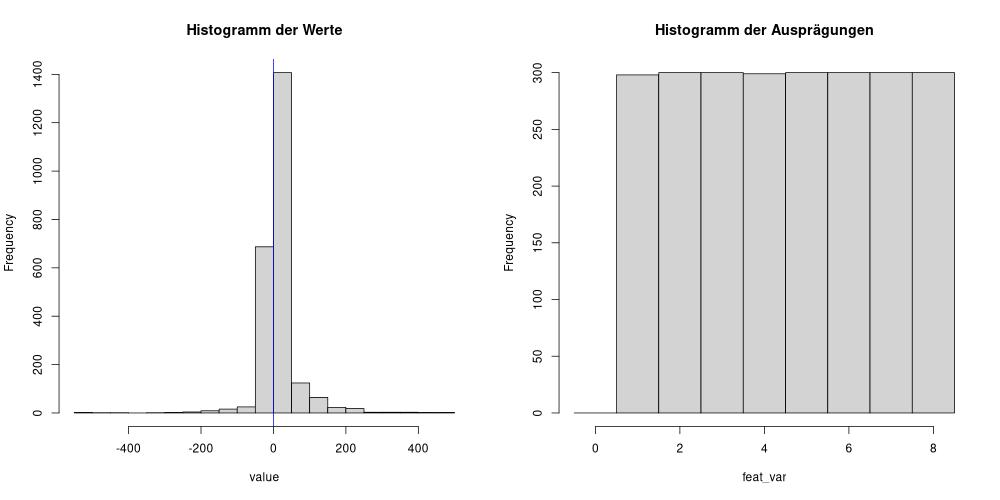
\includegraphics[width=14cm]{"graphiques/hist_feat_value.jpg"}
    \caption{Histogramme d'un èstimateur}
    \label{hist_C_inf}
  \end{center}
\end{figure}


\section{Code Matlab}
\lstinputlisting{mini_projet.m}

\section{Code VBA}
\begin{lstlisting}[
    breaklines=true,
    tabsize=3,
    showstringspaces=false
    extendedchars=\true,
    language={[Visual]Basic},
    frame=single,
    framesep=3pt,%expand outward.
    framerule=0.4pt,%expand outward.
    xleftmargin=3.4pt,%make the frame fits in the text area. 
    xrightmargin=3.4pt,%make the frame fits in the text area.
    ]

Sub Macro1()

Dim T, n, nt, Nd As Integer
Dim r, sigma, S0, t0 As Double

Dim i, j As Integer


r = Range("A2").Value
sigma = Range("A3").Value
T = Range("A4").Value
n = Range("A5").Value
nt = Range("A6").Value
Nd = Range("A7").Value
S0 = Range("A8").Value
t0 = Range("A9").Value

Dim dt As Double
dt = ((T - t0) / n)

' afficher t
Dim temps() As Double
ReDim temps(n + 2)
temps(0) = t0
For j = 1 To n + 2
    temps(j) = temps(j - 1) + dt
Next

Range("I3:I" & UBound(temps) + 1) = WorksheetFunction.Transpose(temps)

Dim S() As Double
ReDim S(1 To n + 1, 1 To nt)
Dim dW As Double
Dim dS As Double
Dim x As Double

'effacer S() aine

'simuler S pas a pas
For j = 1 To nt
    x = S0
    i = 1
    Cells(2 + i, 9 + j).Value = x 'S(i, j) ' copier s dans la worksheet
    Cells(1 + i, 9 + j).Value = "series " & j
    For i = 1 To n + 1
        If i > 1 Then
            dW = Sqr(-2 * Log(Rnd())) * Cos(6.283185307 * Rnd()) * Sqr(dt)
            'dS = S(i - 1, j) * (r * dt + sigma * Sqr(S(i - 1, j)) * dW)
            'aine = Cells(1 + i, 10 + j).Value
            dS = x * (r * dt + sigma * Sqr(x) * dW)
            'S(i, j) = S(i - 1, j) + dS
            x = x + dS 'S(i - 1, j) + dS
            Cells(2 + i, 9 + j).Value = x  'S(i, j) ' copier s dans la worksheet
        End If
        S(i, j) = x
    Next
Next

'Range("J21:O100") = S()


' insert Chart
'Dim Cht As Chart
'Set Cht = Charts.Add
'With Cht
'    .SetSourceData Source:=Sheets("Sheet1").Range("A1:B6")
'    .ChartType = xl3DArea
'End With


MsgBox "Simule pour " & nt & " trajectoires."

'Sheets("Dashboard").Activate
'Range("Parametres").Select
'Range("A13").Value = T

End Sub

\end{lstlisting}



\end{document}
